\section{Быстрое преобразование Фурье}
Быстрое вычисление значений многочлена в точках:
два способа задания многочленов
--- коэффициентами и значениями в точках;
вычисление значений многочлена в точках методом
<<разделяй и властвуй>>;
дискретное преобразование Фурье;
быстрое преобразование Фурье.
Интерполяция: интерполяция в терминах матриц;
матрица Вандермонда;
интерполяция как домножение на обратную матрицу.
Необходимые факты линейной алгебры.

\subsection{Конспект}
Многочлен степени $d$ однозначно задаётся $d + 1$ точкой,
доказательство --- метод интерполяции.
Произведение двух многочленов степени $d$ ---
многочлен степени $2d$.

Заметим, что если мы выбираем точки вида
$x_{2k} = -x_{2k - 1}$,
то можно разделить многочлен
$P(x) = a_0 + a_1 x + a_2 x^2 + \ldots$
в виде $P(x) = P_0(x) + x \cdot P_1(x)$,
где $P_0(x) = a_0 + a_2 x^2 + \ldots$,
а $P_1(x) = a_1 + a_3 x^2 + \ldots$.
Тогда можно посчитать $P(x)$ и $P(-x)$ вместе:
\begin{align*}
    P(x) & = P_0(x) + x \cdot P_1(x) \\
    P(-x) & = P_0(-x) - x \cdot P_1(-x) = \\
    & = P_0(x) - x \cdot P_1(x) \\
\end{align*}

Именно так работает быстрое преобразование Фурье,
только $x$ берутся нетривиальными корнями из 1.
Обычно --- в комплексных числах:
\begin{center}
    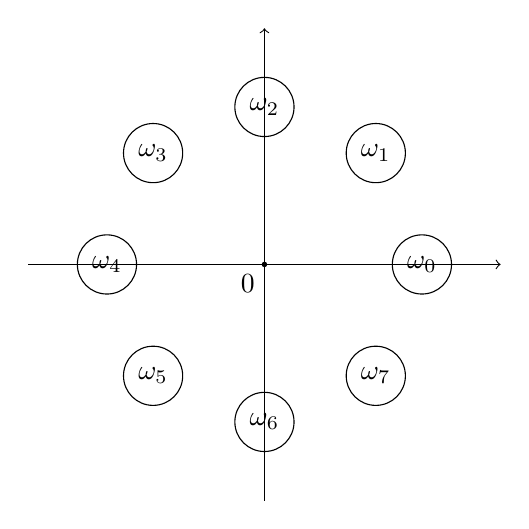
\begin{tikzpicture}
        \foreach \w in {0,...,7} {
            \node[draw,circle] (w\w) at (45*\w : 2cm) {$\omega_{\w}$};
        }
        \draw[->] (-3,0) -- (3,0);
        \draw[->] (0,-3) -- (0,3);
        \fill (0,0) circle (1pt);
        \node[anchor=north east] at (0,0) {$0$};
    \end{tikzpicture}
\end{center}

То есть для $j = 2k \Mod n$
выполняется $\omega_j = \omega_k^2$
и $n = 2^q$.
Иными словами,
$\omega_i = \exp \parens{\frac{2 \pi i}{n}}$.

FFT позволит быстро посчитать точки:

\noindent
\begin{minipage}{\textwidth}
    \begin{algorithmic}
        \State $\omega_N(i) = \exp \parens{\frac{2 \pi i}{N}}$
        \Function{fft}{$n=N, k=0, \Delta=1$}
            \Comment{$k$ --- индекс, $\Delta$ --- шаг индекса}
            \If{$n = 1$}
                \Return $P[k]$
            \EndIf
            \State $P_0(\omega^{2j}) = \Call{fft}{n / 2, k, 2 \Delta}$
            \State $P_1(\omega^{2j}) = \Call{fft}{n / 2, (k + \Delta) \Mod N, 2 \Delta}$
            \For{$j = 0, \ldots, n - 1$}
                \State $P(\omega^j) = P_0(\omega^{2j}) + \omega^j \cdot A_1(\omega^{2j})$
            \EndFor
            \Return $P(\omega^j)$
        \EndFunction
    \end{algorithmic}
\end{minipage}

Очевидно, \textsc{fft} работает за $\O(N \log N)$.

Матричный вид, т.н. матрица Вандермонда:

\[
    \begin{bmatrix}
        P(x_0) \\
        P(x_1) \\
        \ldots \\
        P(x_{n - 1}) \\
    \end{bmatrix}
    =
    \begin{bmatrix}
        1 & x_0 & x_0^2 & \ldots & x_0^{n - 1} \\
        1 & x_1 & x_1^2 & \ldots & x_1^{n - 1} \\
        & & \vdots & & \\
        1 & x_{n - 1} & x_{n - 1}^2 & \ldots & x_{n - 1}^{n - 1} \\
    \end{bmatrix}
    \cdot
    \begin{bmatrix}
        a_0 \\
        a_1 \\
        \ldots \\
        a_{n - 1} \\
    \end{bmatrix}
\]

Интерполяцию можно реализовать домножением на обратную матрицу:
\[
    \frac{1}{n}
    \cdot
    \begin{bmatrix}
        1 & 1 & \ldots & 1 \\
        \omega_0^{-1} & \omega_1^{-1} & \ldots & \omega_{n - 1}^{-1} \\
        \omega_0^{-2} & \omega_1^{-2} & \ldots & \omega_{n - 1}^{-2} \\
        & & \vdots & & \\
        \omega_0^{1 - n} & \omega_1^{1 - n} & \ldots & \omega_{n - 1}^{1 - n} \\
    \end{bmatrix}
    \cdot
    \begin{bmatrix}
        1 & \omega_0 & \omega_0^2 & \ldots & \omega_0^{n - 1} \\
        1 & \omega_1 & \omega_1^2 & \ldots & \omega_1^{n - 1} \\
        & & \vdots & & \\
        1 & \omega_{n - 1} & \omega_{n - 1}^2 & \ldots & \omega_{n - 1}^{n - 1} \\
    \end{bmatrix}
    = ?
\]

Рассмотрим отдельную ячейку $i, j (i \ne j)$:
\[
    \frac{1}{n}
    \sum_{k=0}^{n - 1}
    \omega_k^{-i}
    \cdot
    \omega_k^j
    =
    \frac{1}{n}
    \sum_{k=0}^{n - 1}
    \omega_1^{k(j - i)}
    =
    \frac{1}{n}
    \cdot
    \frac{1 - \omega_1^{n(j - i)}}{1 - \omega_1^{j - i}}
    =
    0
\]

\[
    \frac{1}{n}
    \sum_{k=0}^{n - 1}
    \omega_k^{-j}
    \cdot
    \omega_k^j
    =
    1
\]

Т.е. на главной диагонали единицы,
в остальных ячейках нули.
Получили обратную матрицу.
